    \documentclass{article}

% if you need to pass options to natbib, use, e.g.:
%     \PassOptionsToPackage{numbers, compress}{natbib}
% before loading neurips_2019

% ready for submission
% \usepackage{neurips_2019}

% to compile a preprint version, e.g., for submission to arXiv, add add the
% [preprint] option:
%     \usepackage[preprint]{neurips_2019}

% to compile a camera-ready version, add the [final] option, e.g.:
\usepackage[]{neurips_2019}

% to avoid loading the natbib package, add option nonatbib:
%     \usepackage[nonatbib]{neurips_2019}
\usepackage{float}
\usepackage[utf8]{inputenc} % allow utf-8 input
\usepackage[T1]{fontenc}    % use 8-bit T1 fonts
\usepackage{hyperref}       % hyperlinks
\usepackage{url}            % simple URL typesetting
\usepackage{booktabs}       % professional-quality tables
\usepackage{amsfonts}       % blackboard math symbols
\usepackage{nicefrac}       % compact symbols for 1/2, etc.
\usepackage{microtype}      % microtypography
\usepackage{authblk}
\usepackage{graphicx}
\usepackage{amsmath}
\usepackage{amssymb}
\title{News Recommendation Engine}

\author[1]{Ankita Pal\thanks{A.apal1994@uw.edu}}
\author[1]{Chavi Gupta\thanks{B.chavig@uw.edu}}
\author[1]{Medha Sagar\thanks{C.sagarme@uw.edu}}
\affil[1]{Department of Data Science, University of Washington}

\renewcommand\Authands{ and }

\begin{document}
\maketitle

\begin{abstract}
    The goal of this project is to build a News Recommender System. We chose to work on a News Recommender system since we were interested in addressing both the dimensionality (associated with large text content) and recommendation problems that were covered in class. Among the different domains of recommender systems, news recommendation has been explored relatively less due to the lack of structured data and features. Text mining for news articles using NLP techniques in itself is a different class of problem. In this project we aim to build a pipeline for extracting user and news article features, and eventually build a hybrid recommender system to address the problems of cold start, data sparcity and scalability. 
\end{abstract}

\section{Introduction}

\textit{"Too many cooks spoil the broth"}~Jane Austen. Today the world is flooded and overwhelmed with news. According to MarketingProfs, more than 2 million articles are published everyday on the web. Finding the suitable article a user wants to read, in this overwhelming amount of news, would be a very tedious job in this scenario. Therefore, we decided to take up the development of a news recommendation engine. This recommendation engine uses user side information as well as the news article information and then passes it through a Collobarative Filtering and Content Based Filtering(CF-CBF), to recommend a news article to the user. We use hierarchical clustering to group the users into clusters based on the number of retweets. We use hierarchical Latent Dirichlet allocation (LDA) to find the most relevent topics within the news articles. The (CF-CBF) takes the results from these the clustering and LDA process and recommends a new-article based on the choice of the individual and topic of the article.

\section{Relevant Work}

Amidst all the research done for recommendation systems, new recommendations have been one of the most challenging and relatively unexplored problems. In the domain of news recommender systems, there are 3 classes of recommendation algorithms- Collaborative Filtering (CF), Content-based Filtering (CBF) and hybrid algorithms. The paper \cite{ref1}, proposes the use of building a hybrid recommendation algorithm. They view the problem in 2 phases - Modeling phase and Recommendation phase. The objective of the modelling phase is to pre-learn user and content models that serve to reduce the dimensionality as well as group similar users/articles together. These modellings are performed offline and stored prior to the recommendation phase. The recommendation phase occurs in real-time where based on a reader query, the results of the CF and CBF approaches are combined together to produce a set of recommendations. \\  
In paper \cite{CBFpaper}, the authors propose an interesting approach to calculate the recommendation score for the content filtering algorithm. The authors propose to compute the user’s interest in a category (or topic) based on the user’s overall interest in a topic and also the trend of interest for a topic over time. By combining these “long-term” and “short-term” effects, we can estimate the current interest of a user for a topic. In this project we will use a similar approach for the CBF recommendation. \\
The paper \cite{userClustering} recommends using retweet information to cluster tweets instead of tweet text. The reason was that the tweets are usually restricted to 280 characters and words are often abbreviated (modern text language) and contain special symbols like hashtags and emojis. Thus the paper proposed to calculate the similarity between tweets based on the overlap rate of users who retweeted them, creating a retweet network followed by clustering the tweets based on network clustering.  In this project we decided to use a similar approach to cluster the users based on a retweet network. This user modelling will be used in the CF recommendation approach. \\
Eventually to combine the recommendations, we will explore the use of a weighted additive recommendation score or a multiplicative score as proposed in \cite{CBFpaper}.

\section{Data Collection}

In order to create a news recommendation engine, we needed news as well as user data to model the user-item interactions. While there are many text corpuses for news article data, our literature surveys showed that there are no readily available data sources to collect user interactions with news items. 

Therefore, we decided to use Twitter data to understand how users interact with digital news entities on Twitter. 
The twitter data used in our project was collected using the FakeNewsNet data repository. The repository contains information about tweets that contain news article information. These news articles are shared on Twitter via tweets and/or re-tweets. The repository collects news articles from two predominant websites:
\begin{enumerate}
\item GossipCop
\item Politifact
\end{enumerate}

For the course of this project, we are focussing on news articles supplied by Politifact. Politifact is a non-profit fact checking website reporting on the accuracy of statements made by elected officials, candidates, their staffs, lobbyists, interest groups and others involved in U.S politics. The articles supplied by Politifact are predominantly related to the U.S Politics. 

We will be using the news articles and its metadata collected by Politifact to extract features from the news articles. Additionally, we will be studying the tweets and the retweets of the articles to extract features that would be helpful in modeling user behavior. \\

\subsection{Data Collection Process}:
Our data collection process can be divided into two phases.

\subsubsection{Phase I : Twitter Data Collection}
Our data collection process starts by using the FakeNewsNet repository to collect information about news articles supplied by Politifact. Twitter API keys are used for collecting data from Twitter.
Each news article has the following information:

\begin{enumerate}
\item Article ID : unique identifier of a news text
\item Article Text: the text of the article
\item Article URL: the link to the article
\item Article Keywords: keywords from the article
\item Article Published On: date on which the article was published
\item Tweet Info:
\begin{itemize}
\item Tweet ID: unique identifier for the tweet that contains the article
\item Tweet Timestamp: timestamp when tweet was tweeted
\item Tweet Retweet: no. of time the tweet was retweeted
\item Tweet favorite: no. of timed tweet was favorited
\item User Info:
\begin{itemize}
\item User ID: unique identifier for the user who tweeted about the article
\item User Location: location of the user
\item Follower Count: no. of followers the user has
\item Friend Count: no. of friends the user has
\item User Favourite Count: no. of favorite tweets
\item User Status Count: user statuses count
\end{itemize}
\end{itemize}
\item Retweet Info:
\begin{itemize}
\item Retweet ID: Unique Identifier for the retweet
\item Retweet timestamp: timestamp when tweet was tweeted
\item Retweet UserID: unique identifier of the user who retweeted the tweet
\item User Info:
\begin{itemize}
\item User ID: unique identifier for the user who tweeted about the article
\item User Location: location of the user
\item Follower Count: no. of followers the user has
\item Friend Count: no. of friends the user has
\item User Favourite Count: no. of favorite tweets
\item User Status Count: user statuses count
\end{itemize}
\end{itemize}
\end{enumerate}

\begin{figure}[H]
    \centering
    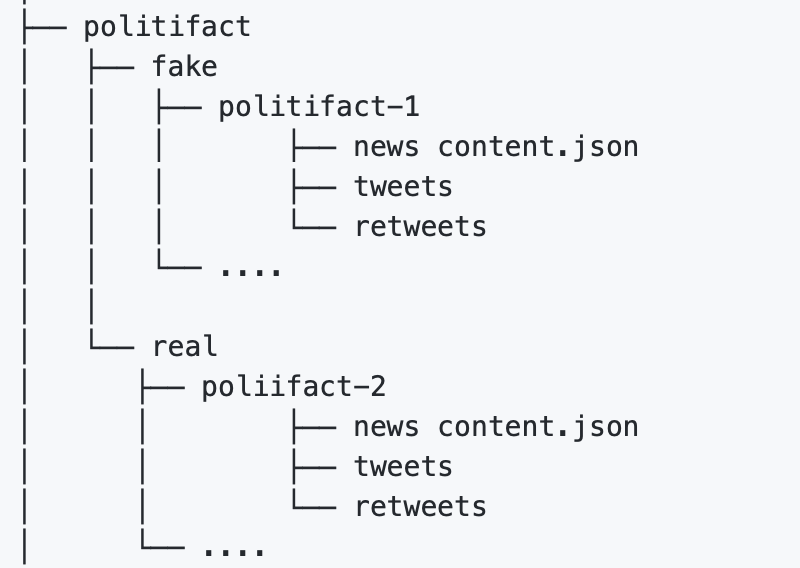
\includegraphics[scale=0.5]{NeuRIPS2019/fakenews.png}
    \caption{Data Hierarchy}
    \label{Data Hierarchy}
\end{figure}
\subsubsection{Phase II : News Article Collection}
In order to collect data for modeling the news article text, we used ‘All the News’ dataset on Kaggle which contains 143,000 news articles from 15 different American publications. 
The motivation to use additional news data was to make a generalizable model for feature extraction on the textual article data.

\begin{figure}[H]
    \centering
    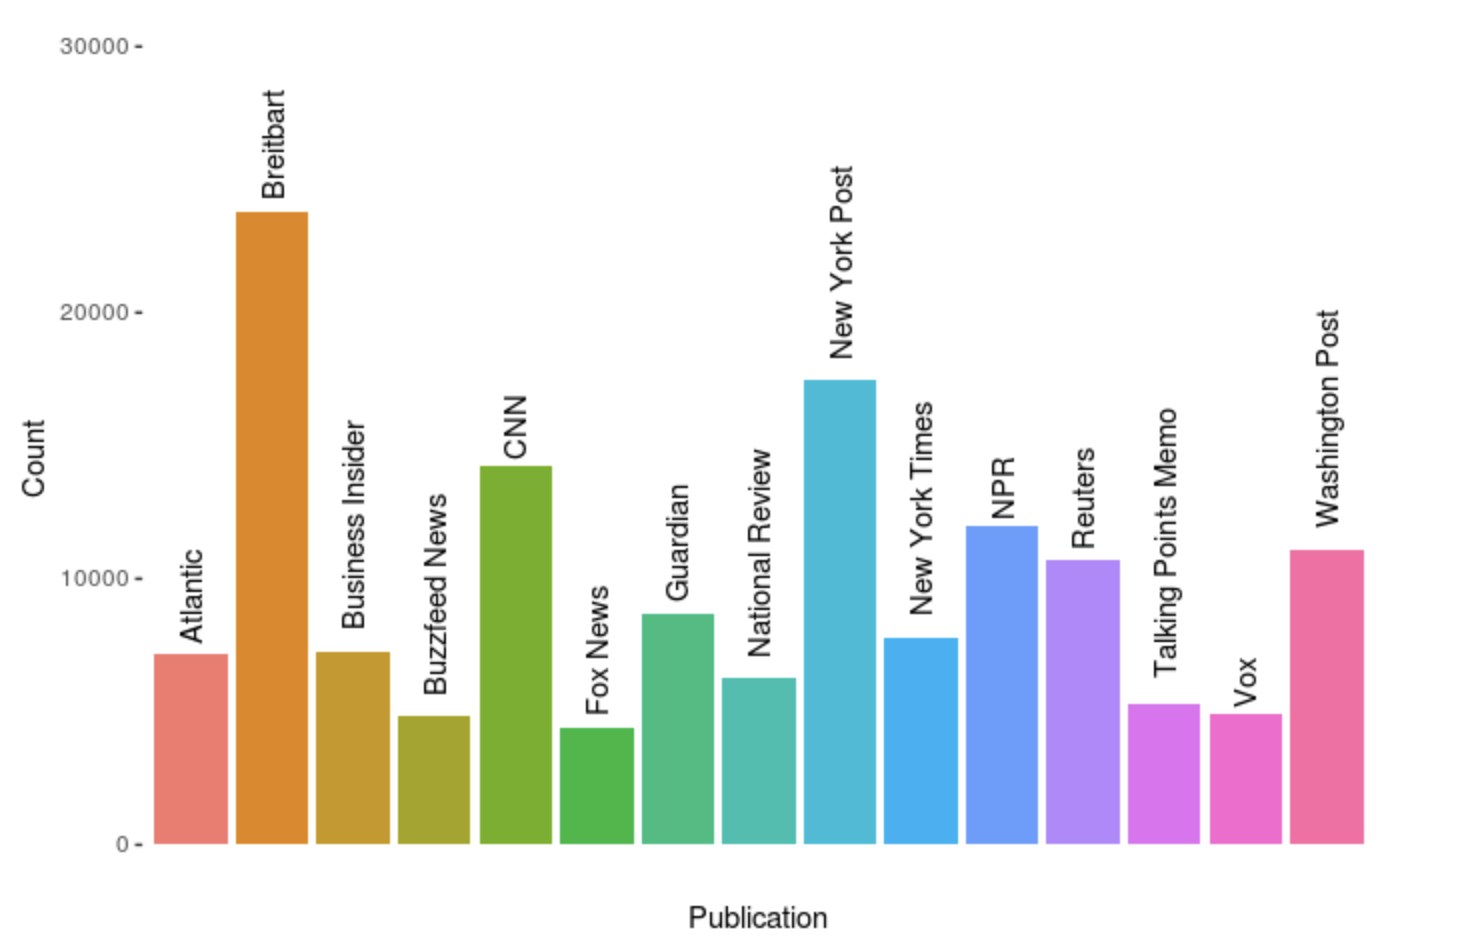
\includegraphics[scale=0.5]{NeuRIPS2019/all-the-news.png}
    \caption{Distribution of News Articles and Publication}
    \label{Distribution of News Articles and Publication}
\end{figure}

\textbf{Data Statistics}:
Since, the data downloading time and the time required to parse the tweets is exorbitant, we report the following statistics as it stands:

\begin{enumerate}
\item Total Number of Articles: 564
\item Total Number of Articles Processed: 285
\item Total Number of Tweets Processed: 239051
\item Total Users Processed Processed: 155353
\item Average Number of Tweets Per User: 3
\end{enumerate}\\

\textbf{Challenges:}\\
\textbf{1. Absence of publicly available data}: As mentioned above, after rigorous literature review we realized that while there are many text corpora for news articles, there does not exist any publicly available dataset that captures the user interactions with news articles. Therefore, we had to create a dataset from scratch to collect the user interactions and news articles. We decided to leverage Twitter data to solve this problem. We have used tweets and retweets as a measure of interaction between users and digital news articles on Twitter.

\textbf{2. Large Amount of Hierarchial Data}: For the scope of this project, we decided to just use Politifact news articles to model our recommendation engine. For a total of 564 news articles, we realized that the due to the hierarchical nature of Twitter data, the user-item interactions are huge. For example, for one article, we can have as many as 30,000 tweets for which we need to parse both the user information and the tweet information. Each of these 30,000 tweets can further have hundreds of retweets. Those retweets would again have to be aggregated along with their author information to create dense user networks. This leads to huge processing times to construct the data. In order to overcome the high computing cost, we are running our analysis and parsing using Google Cloud Platform.

\textbf{2. Skew in News Articles}: Since, we are just using Politifact articles, we realized that creating LDA models using just the Politics related articles might lead to non-generalize results. T  


\section{Exploratory Data Analysis}

We start our EDA with the analysis of our news articles. We have a collection of 515 articles. For our EDA, we aim to analyse the topics present in our news articles data. \\
 For this, we train our data from an external data source and then analyse how it categorises the news articles. The data process for the same is: \\

\begin{figure}[H]
\centering
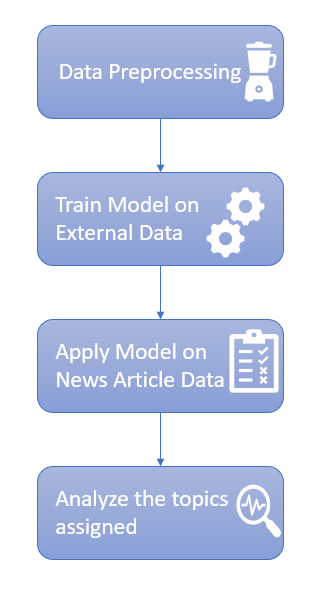
\includegraphics[scale=0.6]{lda_eda_process.PNG}
\caption{Workflow}
\end{figure}

For data prepossessing we use the steps including:
\begin{itemize}
	\item Removal of special characters
	\item Removal of stop words
    \item Making Bigrams 
    \item Lemmatization
\end{itemize}
Our next step was to use this data to model the topics for the external data. We plot the coherence score vs number of topics to help us get the optimum number of topics.

\begin{figure}[H]
    \centering
    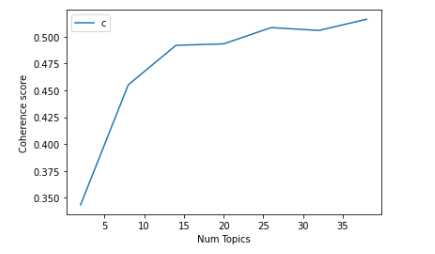
\includegraphics[scale=1.5]{score.PNG}
    \caption{Topic Number vs Coherence Score}
    \label{Topic Number vs Coherence Scorel}
\end{figure}

We notice that the optimum number of topics is 15. We create a LDA model with this hyper parameter. We get the following topics and the corresponding word weights.

\begin{figure}[H]
    \centering
    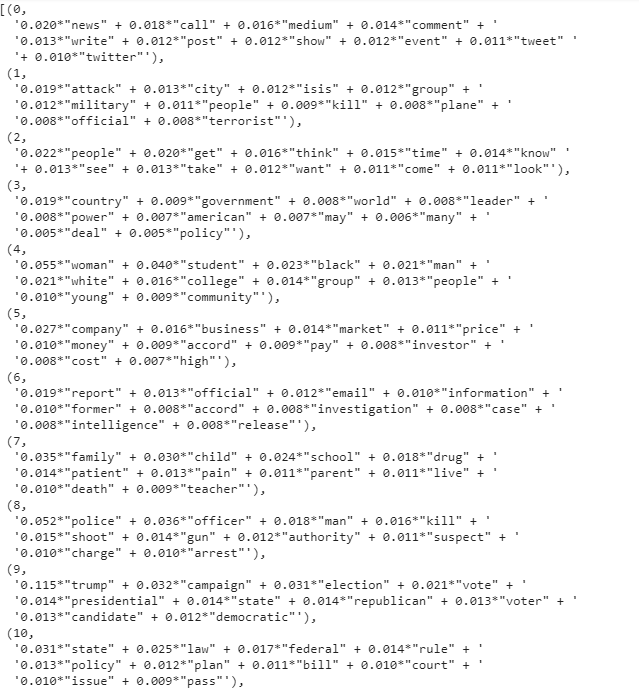
\includegraphics[scale=0.8]{NeuRIPS2019/words.PNG}
    \caption{Word Weightage in Topics}
    \label{Word Weightage in Topics}
\end{figure}

Next we apply the model on the dataset of 515 news articles, to get the predominant topics in the dataset. Assigning the topic to with the maximum score to the document and plotting the count of documents for each topic gives the following graph:

\begin{figure}[H]
    \centering
    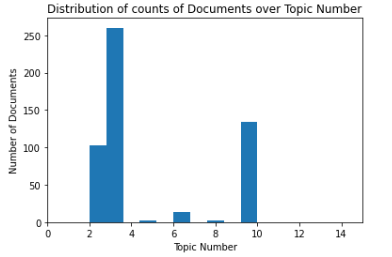
\includegraphics[scale=1]{dist.PNG}
    \caption{Topic number vs Count of documents in news articles data}
    \label{Topic number vs Count of documents in news articles data}
\end{figure}

Thus we see that only 3 of the topics are pre-dominant in our document. By analysis of the keywords we see all three of these topics are related to politics. Also we observe that 2 and 9 are the topic numbers which are most  frequently occurring, which is consistent with Figure \ref{Visualisation to explore topics and keywords}. 

Also, we use k-means to find the distribution of the topics in the news articles data. First to find the optimum number of clusters in the data, we plot a SSE and number of clusters plot. We get the following graph:
\begin{figure}[H]
    \centering
    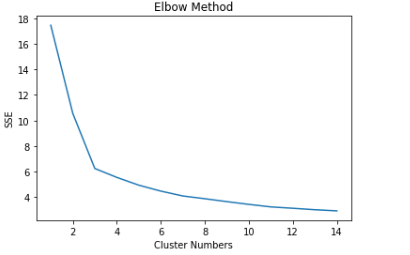
\includegraphics{sse.PNG}
    \caption{Number of clusters vs SSE}
    \label{Number of clusters vs SSE}
\end{figure}

We find that the number of clusters is 3 and this is consistent with the find from figure \ref{Topic number vs Count of documents in news articles data}. The distribution of documents for among the cluster  is:
\begin{figure}[H]
    \centering
    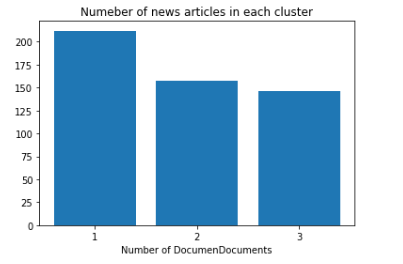
\includegraphics{cluster.PNG}
    \caption{Number of Documents in each cluster}
    \label{Number of Documents in each cluster}
\end{figure}



Thus, we conclude that we need to further divide the topics into sub-topics for analysis.


\section{Algorithm}

\textbf{Understanding the relationship in the data:} The data is composed of users, tweets and news articles. The users are linked to tweets either by directly tweeting the articles or by retweeting the articles. Each tweet refers to a news article. \\

The algorithm is divided into 3 major components. The description of the algorithm for each step is described below:- \\

\subsection{User Interest Modelling (Content-Based Filtering Component)}

\subsubsection{LDA for Topic Modelling}

For this component the first step is to generate classify the news articles into different categories (or topics). The purpose of this is to reduce the dimension space of the news articles and to group similar articles based on text mining. For creating these topics we will use hierarchical topic modelling since the news articles in our dataset are already known to be related to Politics. Thus we classify each news article under a topic $\{c_1, c_2, c_3 \textellipsis \}$. \\

\subsubsection{User’s Genuine News Interest in Time Period $t$}

The genuine interest of a user in a topic (categorized by LDA) is represented as follows:
\begin{equation}
\begin{aligned} 
interest_{u,t}(topic = c_i) 
& = p_t(article | topic = c_i) \\
& = \frac{p_t(topic = c_i| article) p_t(article)}{p_t(topic = c_i)}
\end{aligned}
\end{equation}
Where $p_t(topic = c_i| article) = \displaystyle \frac{\textrm{number of articles tweeted by user in topic $c_i$}}{\textrm{number of articles tweets by user (during time period $t$)}}$, \\
$p_t(article) = \displaystyle \frac{\textrm{number of articles tweeted by user}}{\textrm{total number of articles (during time period $t$)}}$, \\
$p_t(topic = c_i) = \displaystyle \frac{\textrm{number of articles in topic $c_i$}}{\textrm{number of articles during time period $t$}} $.


\subsubsection{Combining interest with past trend}

The overall interest of a user $u$ in topic $c_i$ is: \\
\begin{equation}
\begin{aligned}
interest_u(topic = c_i) 
& = \displaystyle \frac{\sum_{t}(N^t \times interest_{u,t}(topic = t_i)}{\sum_{t} N^t}	 \\
& = \displaystyle\frac{\sum_{t} \left(N^t \times \displaystyle\frac{p_t(topic = c_i| article) p_t(article)}{p_t(topic = c_i)}\right)}{\sum_{t} N^t} \\
\end{aligned}    
\end{equation}

Where $N^t =$ Number of articles tweeted by user in time period t. \\

\subsubsection{Predicting the User’s Current News Interest}

We represent the current time period with subscript $0$. Thus the interest at the current time period is as follows: \\

\begin{equation}
\begin{aligned}
interest_{u,0}(topic = c_i) = \displaystyle\frac{p_0(article | topic = c_i) \times p_0(topic = t_i) }{p_0(article)}
\end{aligned}  
\end{equation}

We estimate $p_0(article | topic = c_i)$ by $interest_u(topic = c_i)$. \\ Also, we assume the the probability of tweeting about any news article is constant. \\

\begin{equation}
\begin{aligned}
\therefore interest_{u,0}(topic = c_i) 
& \propto \displaystyle \frac{interest_u(topic = c_i) \times p_0(topic = t_i)}{p(article)} \\
& \propto \displaystyle\frac{p_0(topic = t_i) \times \sum_{t} \left(N^t \times \displaystyle\frac{p_t(topic = c_i| article)}{p_t(topic = c_i)} \right)}{\sum_{t} N^t}
\end{aligned}
\end{equation}

\subsubsection{Smoothing factor $G$}

If the user is found to tweet very rarely or in the case of a new user (cold-start problem), we would like to approximate a user’s interest based on the current trend. Thus we add a smoothing factor G that act as virtual tweets. If $\sum_{t} N^t$ is much larger than $G$, then the interest approximates to the user’s real interest. However if it is very small, then the interest will approximate to the general current news trend. \\

\begin{equation}
\begin{aligned}
interest_{u,0}(topic = c_i) \propto \displaystyle\frac{p_0(topic = t_i) \times \left(\sum_{t} \left(N^t \times \displaystyle\frac{p_t(topic = c_i| article)}{p_t(topic = c_i)}\right) + G\right)}{\sum_{t} N^t + G }
\end{aligned}
\end{equation}

Thus the Content-Based Filtering Score for a user $u$ and topic $c_i$ is $interest_{u,0}(topic = c_i)$. \\
Note that offline we can precompute $N^t$ and $\displaystyle\frac{p_t(topic =c_i| article)}{p_t(topic = c_i)}$. Thus in real time we only have to calculate the $p_0(topic = c_i)$ i.e. the probability of a topic currently being in trend. \\

\subsection{User clustering (Collaborative Filtering Component)}

For clustering users based on retweet network, we must do the following steps:-

\subsubsection{Create User Retweet Network}

\begin{enumerate}
\item Create a User-Tweet matrix $W$ where $W_{u, t} = \displaystyle\frac{1}{\textrm{number of retweets on the tweet $t$ by user $u$}}$
\item Get user weights by finding the sum of each row in the $W$ matrix. Let this user weight matrix be $UW$.
\item Create a User-User matrix where $U_{u1, u2} = \textrm{(Sum of (1/number of retweets) for each common retweet between user u1 and u2)}$ 
\item Calculate the cosine similarity of each user link as $\displaystyle\frac{U_{u1, u2}}{UW_{u1} \times UW_{u2}}$.
\item Create a graph G based with each user as a node and each edge is the link between each user with edge weight as the cosine similarity and edge value as the number of common retweets.
\item Cluster the graph using the fast greedy algorithm. 
\end{enumerate}

Thus we get groups of users. Using the results of the LDA from the previous section, we can create a matrix $GC$ where $GC_{g, c_i} = \textrm{average of probabilities of category $c_i$ read by the users in user group $g$}$ \\

We finally get the recommendation score based on Collaborative Filtering by using $GC_{g, c_i}$ where user $u$ belongs to user group $g$ and the article belongs to topic $c_i$.
\subsection{Recommendation Generation Component}

From the above two sections we saw how we can compute two recommendation scores for each news article for a user. Let the recommendation scores from the Content-Based Filtering component be $CF$ and Collaborative Filtering component be $CBF$. We can calculate a single recommendation score for each article as $CF \times CBF$. \\

Finally using the recommendation scores for each article for each user, we can recommend the top news articles for any user. \\


\section{Conclusion}

{Description of general difficulties with your problem which bear elaboration
}

\begin{thebibliography}{9}

\bibitem{ref1} Ismail, Walaa \& Nasr, Mona \& Saied, Mohamed. (2018). A HYBRID NEWS RECOMMENDER SYSTEM.

\bibitem{CBFpaper} Liu, J., Dolan, P., & Pedersen, E. R. (2010, February). Personalized news recommendation based on click behavior. In Proceedings of the 15th international conference on Intelligent user interfaces (pp. 31-40).

\bibitem{userClustering} Uchida, K., Toriumi, F., & Sakaki, T. (2017, August). Evaluation of retweet clustering method classification method using retweets on Twitter without text data. In Proceedings of the International Conference on Web Intelligence (pp. 187-194).

\end{thebibliography}
\end{document}
